\section{Evaluation}
\label{evaluation-section}
We evaluate the four \texttt{BEE backends} on four different platforms: For \texttt{BEE-Charliecloud}
%, we use our testbed cluster system Darwin. Each node has two 8-core Intel Ivy Bridge E5-2650 v2 CPUs with 251GB RAM. For
and \texttt{BEE-VM}, we test them on the bare-metal envionment on \texttt{Chameleon Cloud} at Texas Advanced Computing Center (TACC). Each node is equipped with two Intel Xeon E5-2670 v3 CPU (clock frequency at 2.30 GHz) with 128 GB DRAM. Each node is connected with Mellanox ConnectX-3 Infiniband card with peak transfer speed at 10 Gbps.  For \texttt{BEE-AWS}, we choose to use \texttt{c3.4xlarge} EC2 type at AWS Oregon region. Each node is equipped with Intel Xeon E5-2680 v2 CPUs and 30GB DRAM. On \texttt{BEE-OpenStack}, we choose the OpenStack environment at \texttt{Chameleon Cloud}@University of Chicago. We focus on evaluating three kinds of performance that are most important for HPC applications: \textit{computation}, \textit{storage}, and \textit{network}. For each test, the comparison baseline is the native performance provided on each platform without using \texttt{BEE} or any additional encapsulated runtime system. Note: all platforms, except AWS, provide access to the bare-metal hardware, so baseline performance is the native performance on the hardware. For AWS, its Xen-based VM is an inseparable part of the platform and the underlying physical hardware is inaccessible to general users, so its baseline is the performance inside VMs.

\begin{figure*}[t]
    \centering
    \begin{subfigure}[t]{0.49\textwidth}
        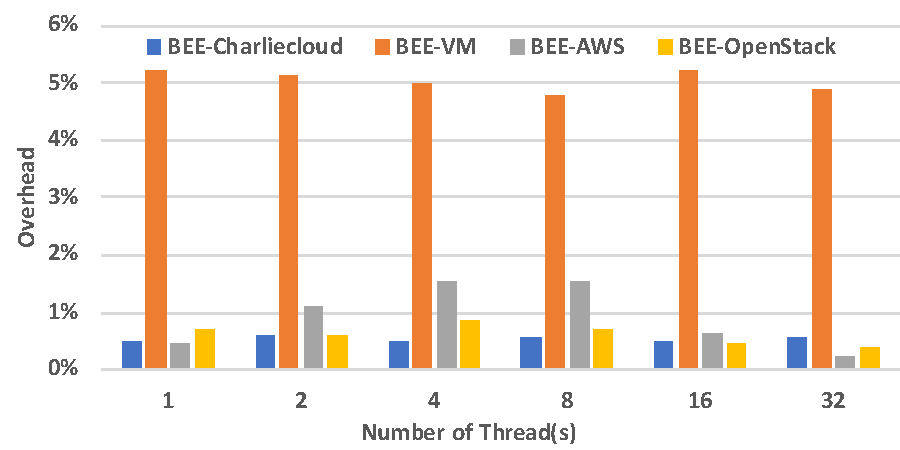
\includegraphics[width=\textwidth]{figures/bt.pdf}
        \caption{Compute intensive workload (BT)}
    \end{subfigure}
    \begin{subfigure}[t]{0.49\textwidth}
        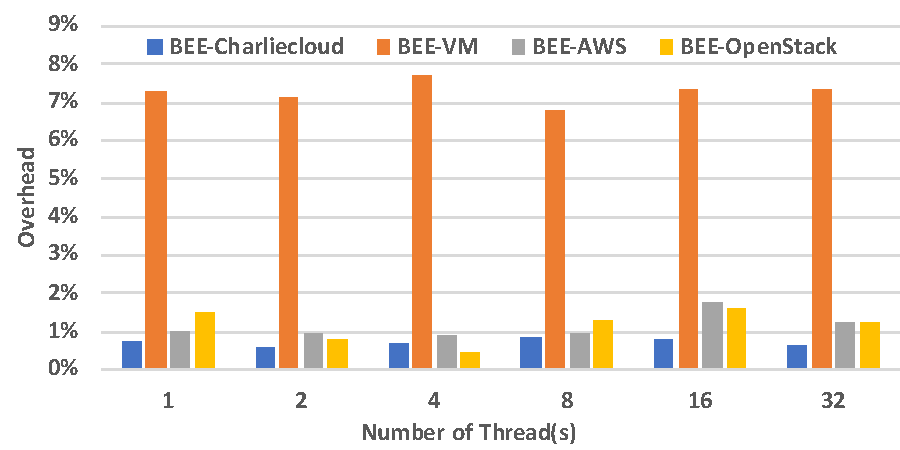
\includegraphics[width=\textwidth]{figures/is.pdf}
        \caption{Memory intensive workload (IS)}
    \end{subfigure}
    \vspace*{-0.5em}
    \caption{Performance overhead compare with native performance provided on each corresponding platform.}
    \label{comp}
    \vspace*{-1em}
\end{figure*}

\begin{figure*}[t]
    \centering
    \begin{subfigure}[t]{0.49\textwidth}
        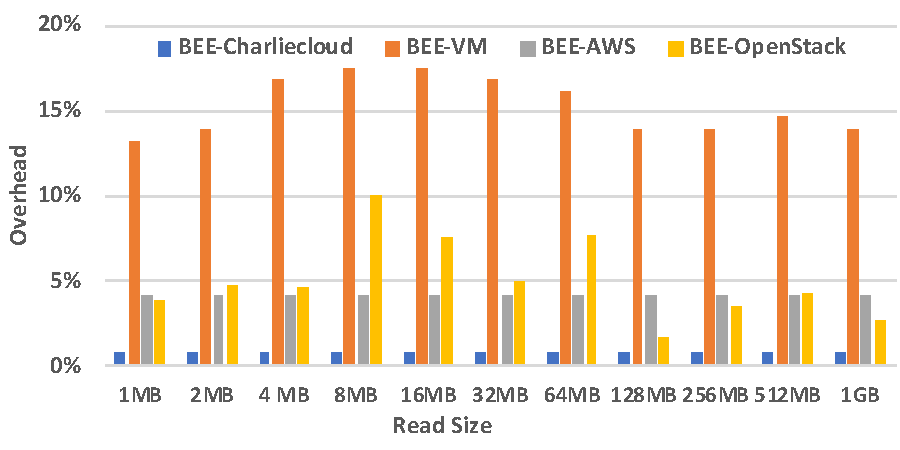
\includegraphics[width=\textwidth]{figures/read.pdf}
        %\caption{Compute intensive workload (BT)}
    \end{subfigure}
    \begin{subfigure}[t]{0.49\textwidth}
        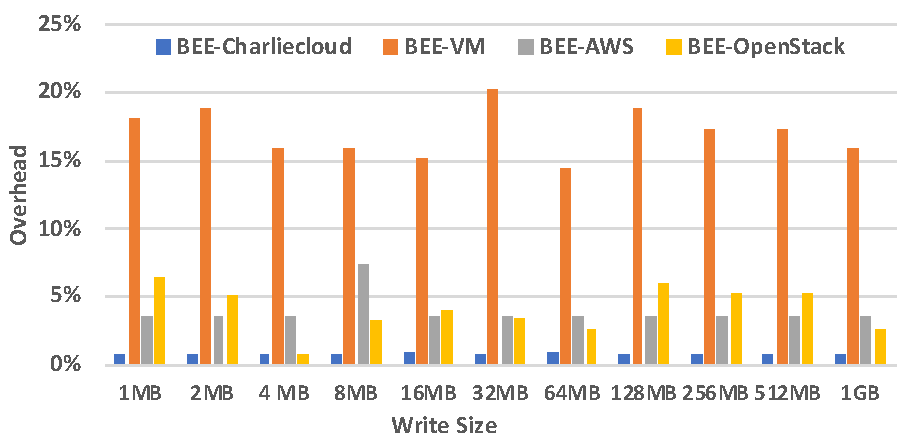
\includegraphics[width=\textwidth]{figures/write.pdf}
        %\caption{Memory intensive workload (IS)}
    \end{subfigure}
    \vspace*{-0.5em}
    \caption{Storage I/O read/write speed overhead compare with native speed provided on each corresponding platform.}
    \label{io}
    \vspace*{-2em}
\end{figure*}



\subsection{Computational Performance}
Computational performance of a platform is one of the most important capabilities for HPC applications. In this section, we compare the computational performance of all four \texttt{BEE backends} with the baseline. We choose one compute intensive benchmark test and one memory intensive benchmark test from the OpenMP version NAS Parallel Benchmarks (NPB)\cite{npb} in our evaluation. We test each benchmark running one to 32 threads (cores) to further show the computational performance on multi-thread environment. 
\subsubsection{Compute intensive workload}
For compute intensive workload, we choose Block Tri-diagonal solver (BT) benchmark test with input matrix size of $102^3$ (problem size: \texttt{class B}).

\begin{comment}
\begin{figure}[t]
    \centering
    \begin{subfigure}[t]{0.24\textwidth}
        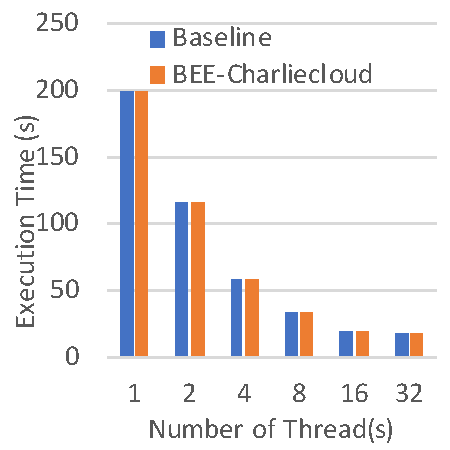
\includegraphics[width=\textwidth]{figures/bt-bee-cc.pdf}
        \caption{\texttt{BEE-Charliecloud}}
    \end{subfigure}
    \begin{subfigure}[t]{0.24\textwidth}
        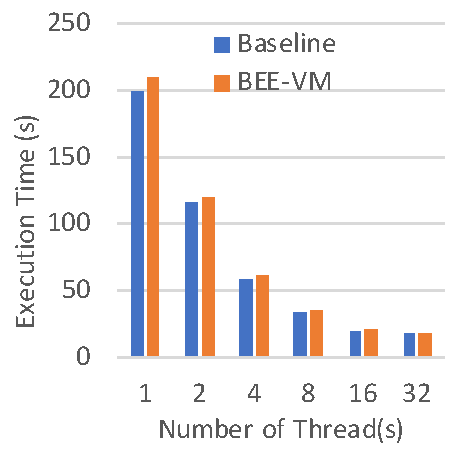
\includegraphics[width=\textwidth]{figures/bt-bee-vm.pdf}
        \caption{\texttt{BEE-VM}}
    \end{subfigure}
    \begin{subfigure}[t]{0.24\textwidth}
        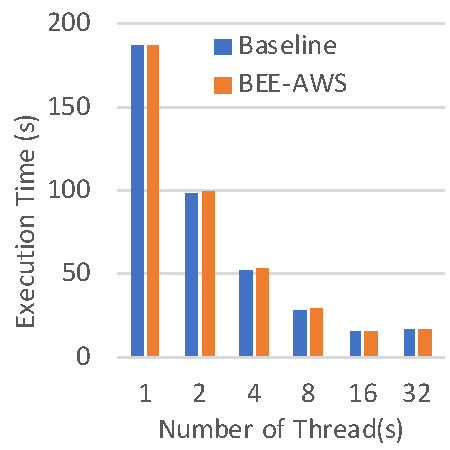
\includegraphics[width=\textwidth]{figures/bt-bee-aws.pdf}
        \caption{\texttt{BEE-AWS}}
    \end{subfigure}
    \begin{subfigure}[t]{0.24\textwidth}
        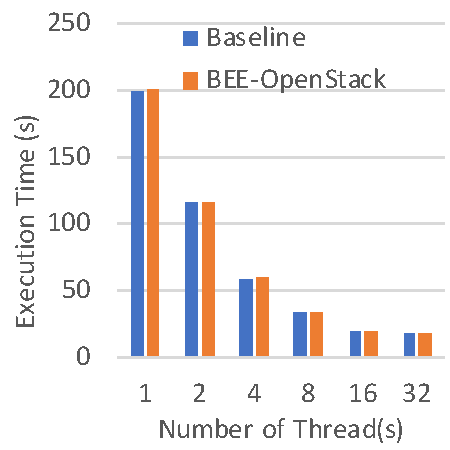
\includegraphics[width=\textwidth]{figures/bt-bee-os.pdf}
        \caption{\texttt{BEE-OpenStack}}
    \end{subfigure}
    %\vspace*{-0.5em}
    \caption{Performance comparison on compute intensive workload (BT).}
    \label{comp}
    %\vspace*{-2em}
\end{figure}
\end{comment}



As we can see in \textbf{Fig. \ref{comp}(a)}, for compute intensive workload, all four \texttt{BEE backends} have low performance overhead: \texttt{BEE-Charliecloud} 0.4\% - 0.6\% (avg. 0.5\%); \texttt{BEE-VM} 4.8\% - 5.2\% (avg. 5.0\%); \texttt{BEE-AWS} 0.2\% - 1.6\% (avg. 0.8\%); \texttt{BEE-OpenStack} 0.3\% - 0.9\% (avg. 0.6\%).
    
\subsubsection{Memory intensive workload}
For memory intensive workload, we choose Integer Sort  (IS) test suit with 134217728 input integer (problem size : \texttt{class C}). 

\begin{comment}


\begin{figure}[t]
    \centering
    \begin{subfigure}[t]{0.24\textwidth}
        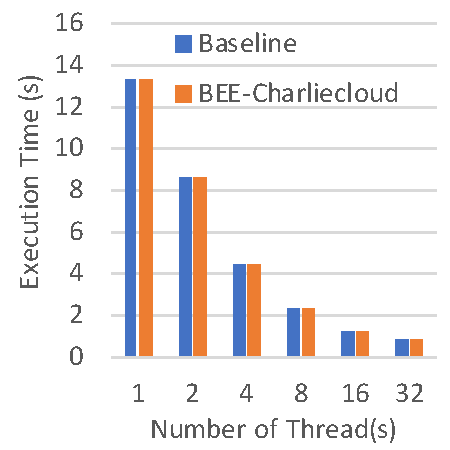
\includegraphics[width=\textwidth]{figures/is-bee-cc.pdf}
        \caption{\texttt{BEE-Charliecloud}}
    \end{subfigure}
    \begin{subfigure}[t]{0.24\textwidth}
        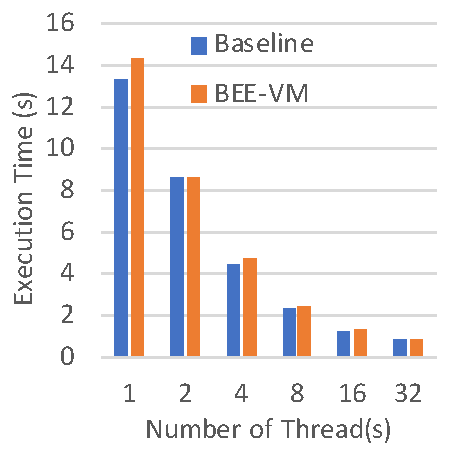
\includegraphics[width=\textwidth]{figures/is-bee-vm.pdf}
        \caption{\texttt{BEE-VM}}
    \end{subfigure}
    \begin{subfigure}[t]{0.24\textwidth}
        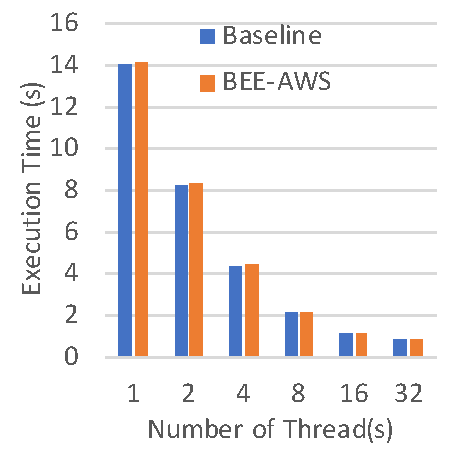
\includegraphics[width=\textwidth]{figures/is-bee-aws.pdf}
        \caption{\texttt{BEE-AWS}}
    \end{subfigure}
    \begin{subfigure}[t]{0.24\textwidth}
        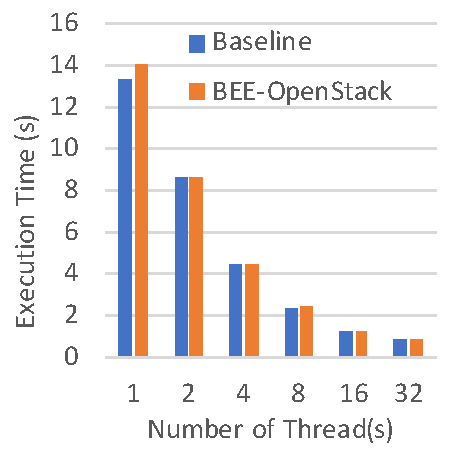
\includegraphics[width=\textwidth]{figures/is-bee-os.pdf}
        \caption{\texttt{BEE-OpenStack}}
    \end{subfigure}
    %\vspace*{-0.5em}
    \caption{Performance comparison on memory intensive workload (IS).}
    \label{mem}
   % \vspace*{-2em}
\end{figure}
\end{comment}


As we can see in \textbf{Fig. \ref{comp}(b)}, for memory intensive workload all four \texttt{BEE backends} also have low performance overhead: \texttt{BEE-Charliecloud} 0.6\% - 0.9\% (avg. 0.7\%); \texttt{BEE-VM} 6.9\% - 7.7\% (avg. 7.1\%); \texttt{BEE-AWS} 0.9\% - 1.8\% (avg. 1.1\%); \texttt{BEE-OpenStack} 0.5\% - 1.7\% (avg. 1.0\%). In addition, both kinds of workload also exhibit similar speedup comparing with their baseline counterparts when we increase the number of threads.

 \begin{figure*}[t]
    \centering
    \begin{subfigure}[t]{0.245\textwidth}
        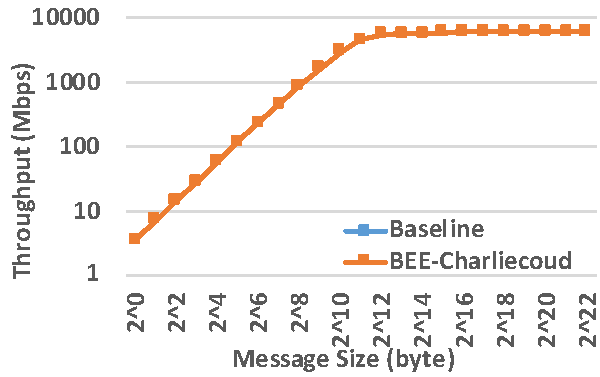
\includegraphics[width=\textwidth]{figures/band-bee-cc.pdf}
    \end{subfigure}
    \begin{subfigure}[t]{0.245\textwidth}
        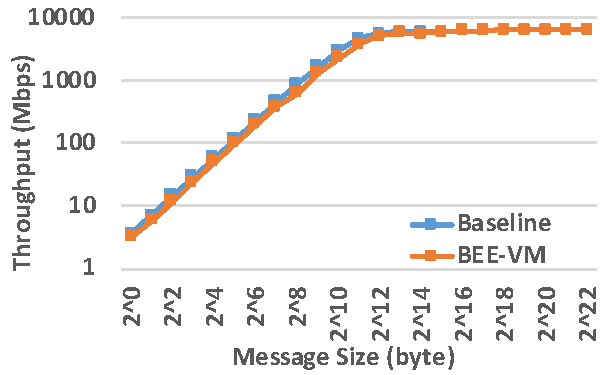
\includegraphics[width=\textwidth]{figures/band-bee-vm.pdf}
    \end{subfigure}
    \begin{subfigure}[t]{0.245\textwidth}
        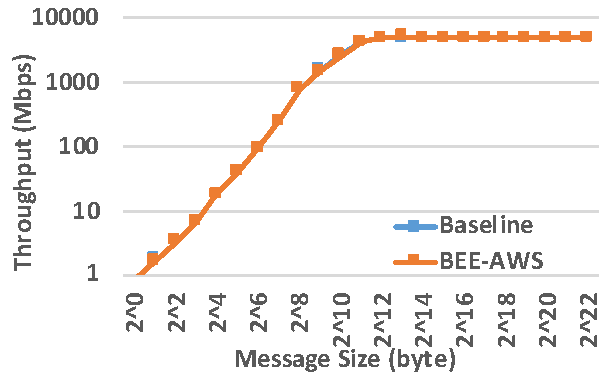
\includegraphics[width=\textwidth]{figures/band-bee-aws.pdf}
    \end{subfigure}
    \begin{subfigure}[t]{0.245\textwidth}
        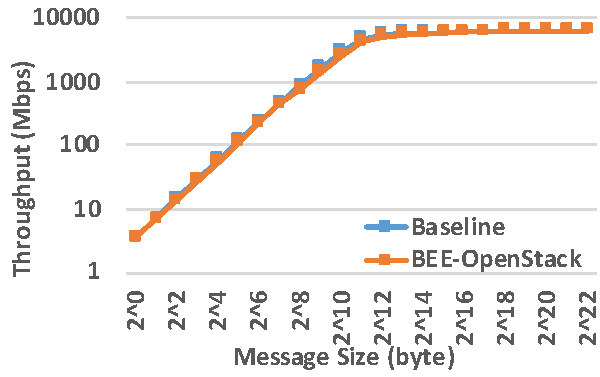
\includegraphics[width=\textwidth]{figures/band-bee-os.pdf}
    \end{subfigure}
    \caption{P2P Network Throughput Comparison}
    \label{net-band}
   % \vspace*{-2em}
\end{figure*}
\begin{figure*}[t]
    \centering
    \begin{subfigure}[t]{0.245\textwidth}
        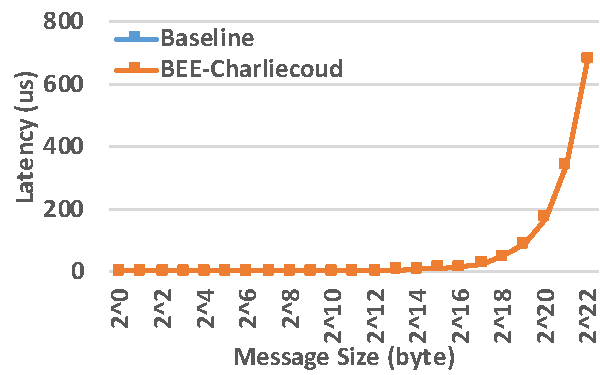
\includegraphics[width=\textwidth]{figures/lat-bee-cc.pdf}
    \end{subfigure}
    \begin{subfigure}[t]{0.245\textwidth}
        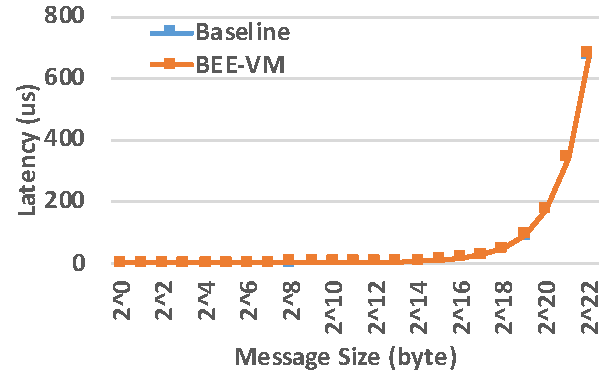
\includegraphics[width=\textwidth]{figures/lat-bee-vm.pdf}
    \end{subfigure}
    \begin{subfigure}[t]{0.245\textwidth}
        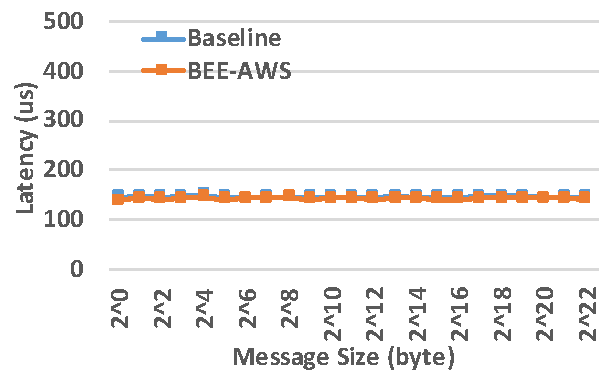
\includegraphics[width=\textwidth]{figures/lat-bee-aws.pdf}
    \end{subfigure}
    \begin{subfigure}[t]{0.245\textwidth}
        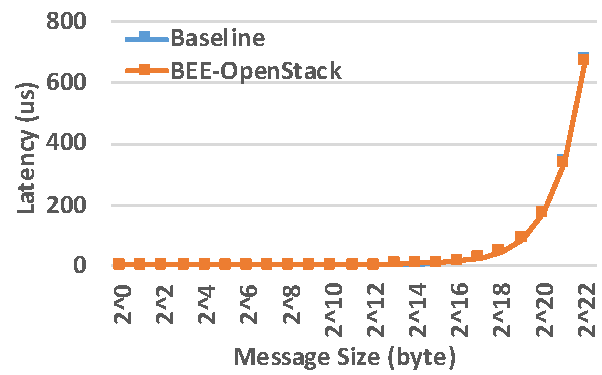
\includegraphics[width=\textwidth]{figures/lat-bee-os.pdf}
    \end{subfigure}
    \caption{P2P Network Latency Comparison}
    \label{net-lat}
   % \vspace*{-2em}
\end{figure*}

\begin{figure*}[t]
    \centering
    \begin{subfigure}[t]{0.245\textwidth}
        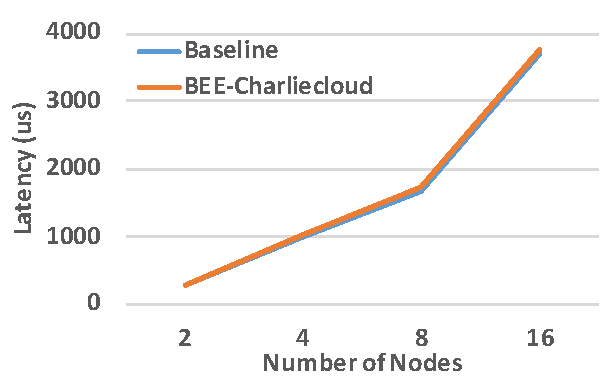
\includegraphics[width=\textwidth]{figures/cl-bee-cc.pdf}
    \end{subfigure}
    \begin{subfigure}[t]{0.245\textwidth}
        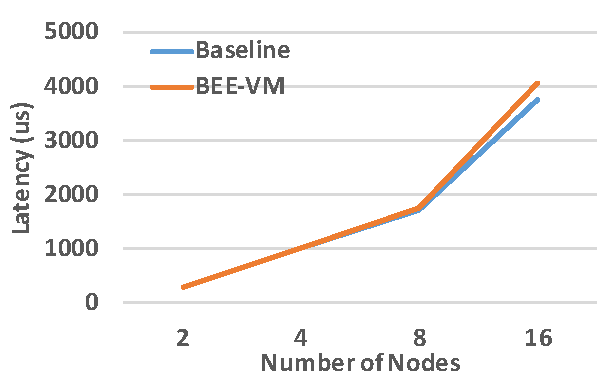
\includegraphics[width=\textwidth]{figures/cl-bee-vm.pdf}
    \end{subfigure}
    \begin{subfigure}[t]{0.245\textwidth}
        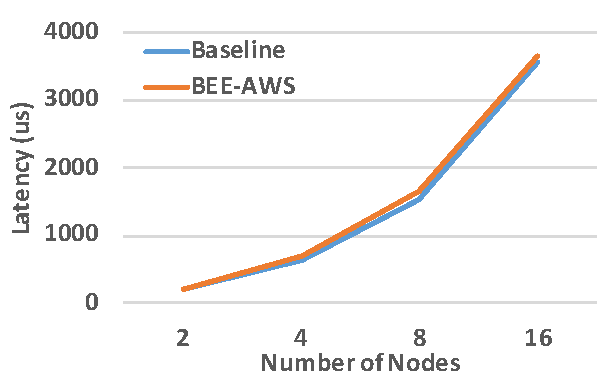
\includegraphics[width=\textwidth]{figures/cl-bee-aws.pdf}
    \end{subfigure}
    \begin{subfigure}[t]{0.245\textwidth}
        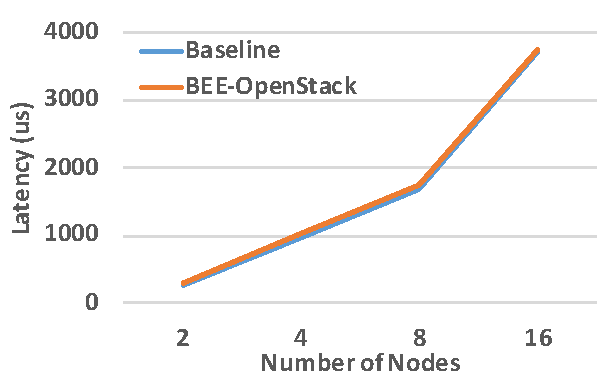
\includegraphics[width=\textwidth]{figures/cl-bee-os.pdf}
    \end{subfigure}
    \caption{All-to-all Network Latency Comparison}
    \label{net-lat-all}
    \vspace*{-2em}
\end{figure*}
\subsection{Storage I/O }
Storage I/O is another key component for many HPC applications. For example, large-scale simulations often need to first load large datasets before computation and frequently dump checkpoints during computation and once the simulation has concluded. Later, these results may be used for other simulations or for analytics. I/O performance plays an important role for the overall performance of HPC applications. 

To evaluate the storage I/O performance of the four \texttt{BEE backends} and compare with the baseline performance, we use the Linux built-in command -- \texttt{dd}. Specifically, to benchmark write performance, we use the \texttt{dd} command to write a file with data from \texttt{/dev/zero}. As for read performance, we use the \texttt{dd} command to read out the file just saved and write to \texttt{/dev/null}. To avoid reading from cache, we use \texttt{echo 3 > /proc/sys/vm/drop\_caches} command to force the system to clear all cached data between each write and read. Usually this file is read-only inside a container, so we issue the command outside the container, achieving the same cache flushing effect. The file used for write and read is placed in the directory that is shared between instances or containers. We test different file sizes ranging from 1 MB to 1 GB. To eliminate noise and variation, we repeat each test 1000 times. \textbf{Fig. \ref{io}} shows the read and write performance on the four \texttt{BEE backends} comparing with the baseline (i.e., the IO performance on each platform without using \texttt{BEE}). As we can see, \texttt{BEE-Charliecloud} produces negligible read and write overhead (~0.08\%). \texttt{BEE-VM} uses both VM and Docker, so it produces relative higher overhead, 13.1\% - 17.5\% (avg. 15.2\%) for read and 15.1\% - 20.1\% (avg. 17.1\%) for write. \texttt{BEE-AWS} produces steady 0.4\% overhead for read and 0.3\% overhead for write. \texttt{BEE-OpenStack} produces 1.7\% - 7.6\% (avg. 5.0\%) for read overhead and 2.7\% - 6.4\% (avg. 4.1\%) for write overhead.

\subsection{Network}
Finally, we evaluate the network performance of the four \texttt{BEE backends}. We use the HPCBench \cite{hpcbench} to measure the bandwidth and latency when transferring data of different sizes between two processes in containers or on the platform without using \texttt{BEE}. \texttt{BEE-VM} and \texttt{BEE-OpenStack} use the Infiniband (IB) on \texttt{Chameleon Cloud} via SR-IOV. \texttt{BEE-Charliecloud} and \texttt{BEE-AWS} use the Ethernet connection. \textbf{Fig. \ref{net-band}} and \textbf{Fig. \ref{net-lat}} show the point-to-point (P2P) network performance. MPI communication function calls between two nodes (one process per node) were used to test the average throughput and latency when transferring different message sizes. It can be seen that all four \texttt{BEE backends} can provide similar network bandwidth and latency compared to the baseline. \textbf{Fig. \ref{net-lat-all}} also show the latencies of all-to-all collective communication in MPI. It shows that all four \texttt{BEE backends} still provide similar network performance large scale. 

%It also shows promising trends on larger clusters. Similar results have been seen in \cite{zhang2016performance}. Note that the Docker container is slightly better than bare-metal in some cases due to the tuning difference under the test scenario.  


\begin{comment}


\begin{figure}[t]
    \centering
    \begin{subfigure}[t]{0.5\textwidth}
        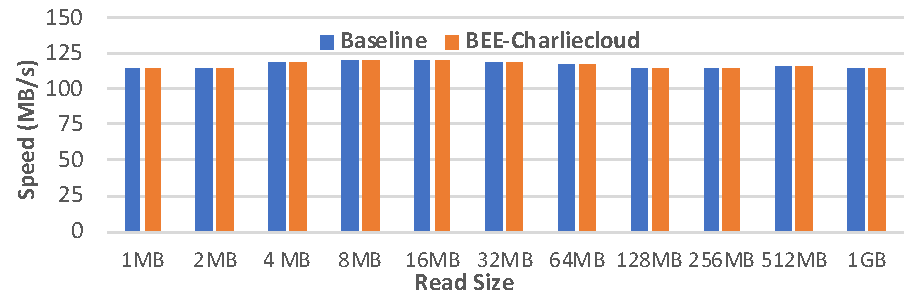
\includegraphics[width=\textwidth]{figures/read-bee-cc.pdf}
        \caption{Read Performance}
    \end{subfigure}
    \begin{subfigure}[t]{0.5\textwidth}
        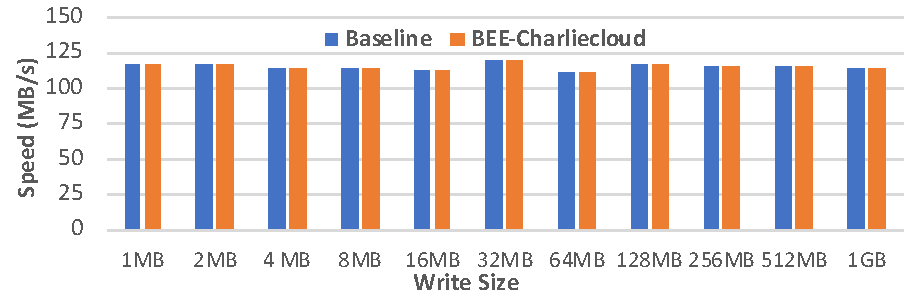
\includegraphics[width=\textwidth]{figures/write-bee-cc.pdf}
        \caption{Write Performance}
    \end{subfigure}
    %\vspace*{-0.5em}
    \caption{Comparison of storage I/O (\texttt{BEE-Charliecloud}).}
    \label{io-cc}
    \vspace*{-0em}
\end{figure}

\begin{figure}[t]
    \centering
    \begin{subfigure}[t]{0.5\textwidth}
        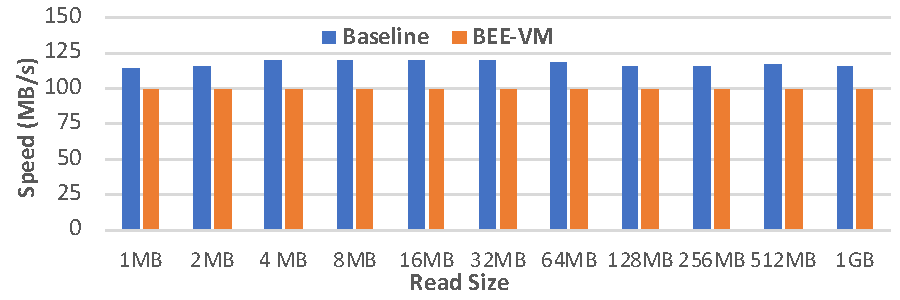
\includegraphics[width=\textwidth]{figures/read-bee-vm.pdf}
        \caption{Read Performance}
    \end{subfigure}
    \begin{subfigure}[t]{0.5\textwidth}
        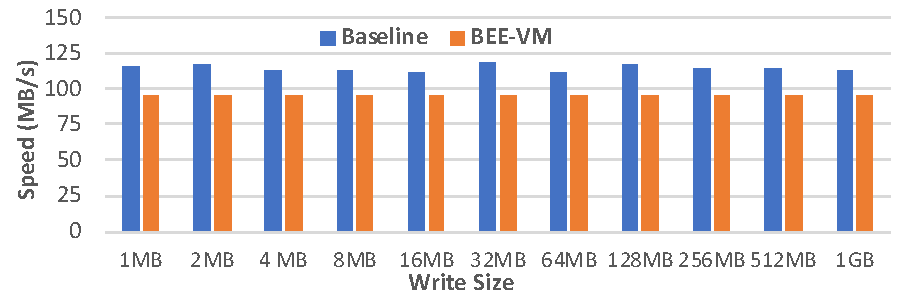
\includegraphics[width=\textwidth]{figures/write-bee-vm.pdf}
        \caption{Write Performance}
    \end{subfigure}
    %\vspace*{-0.5em}
    \caption{Comparison of storage I/O (\texttt{BEE-VM}).}
    \label{io-vm}
   \vspace*{-2em}
\end{figure}

\begin{figure}[t]
    \centering
    \begin{subfigure}[t]{0.5\textwidth}
        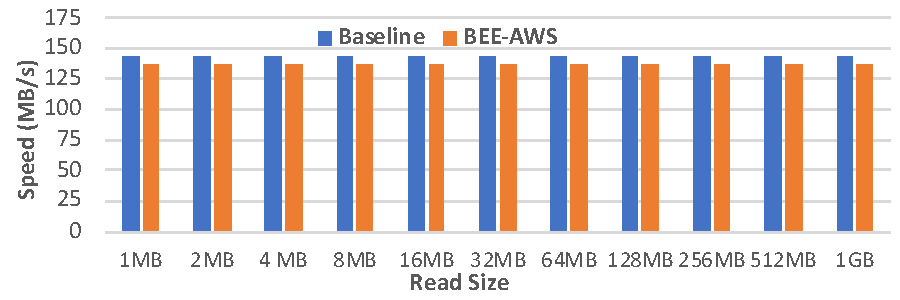
\includegraphics[width=\textwidth]{figures/read-bee-aws.pdf}
        \caption{Read Performance}
    \end{subfigure}
    \begin{subfigure}[t]{0.5\textwidth}
        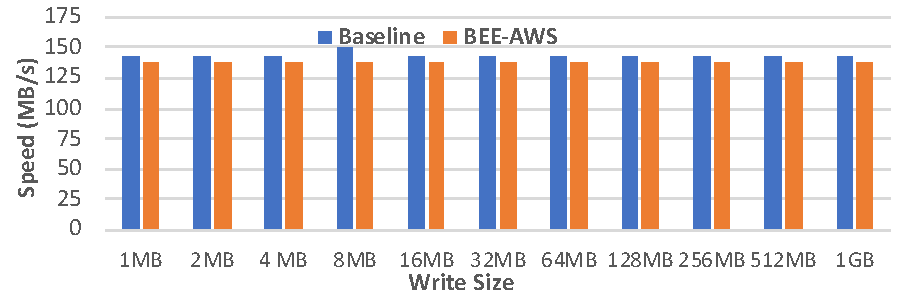
\includegraphics[width=\textwidth]{figures/write-bee-aws.pdf}
        \caption{Write Performance}
    \end{subfigure}
    
    %\vspace*{-0.5em}
    \caption{Comparison of storage I/O (\texttt{BEE-AWS}).}
    \label{io-aws}
   % \vspace*{-2em}
\end{figure}

\begin{figure}[t]
    \centering
    \begin{subfigure}[t]{0.5\textwidth}
        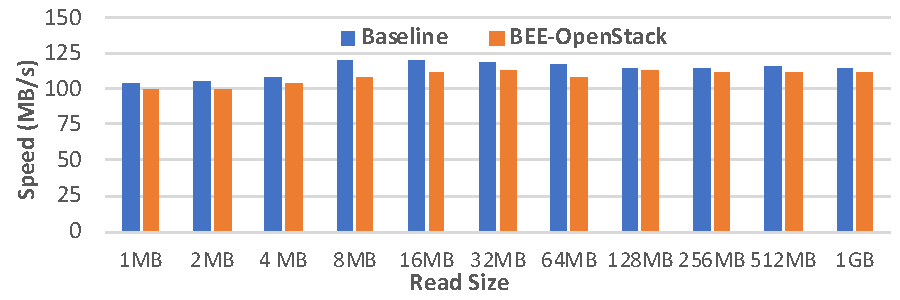
\includegraphics[width=\textwidth]{figures/read-bee-os.pdf}
        \caption{Read Performance}
    \end{subfigure}
    \begin{subfigure}[t]{0.5\textwidth}
        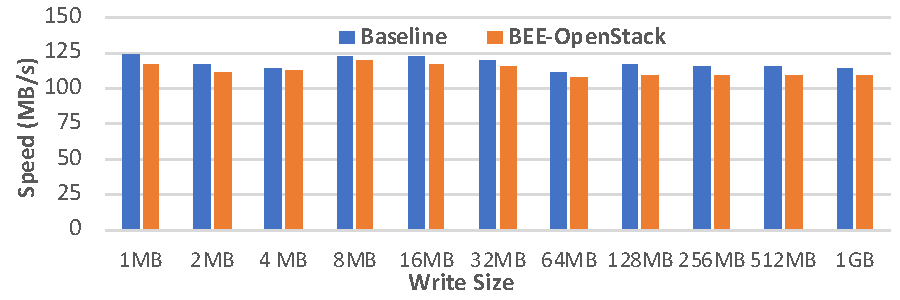
\includegraphics[width=\textwidth]{figures/write-bee-os.pdf}
        \caption{Write Performance}
    \end{subfigure}
    %\vspace*{-0.5em}
    \caption{Comparison of storage I/O (\texttt{BEE-OpenStack}).}
    \label{io-os}
   % \vspace*{-2em}
\end{figure}


\end{comment}




